\chapter{Abbildung der empfangenen Daten auf ein Eingabegerät}
Nachdem die Daten des eingebetteten Systems zur Rollstuhl-Software übermittelt wurden, müssen diese nun auf auf ein herkömmliches Eingabegerät abgebildet werden.
Es wird sich der Frage gewidmet, welches Eingabegerät in Frage kommt und wie möglichst viele, präzise Eingaben auf dieses Eingabegerät abgebildet werden können.
Im letzten Teil des Kapitels werden aufgenommene Datenreihen untersucht, um fehlerhafte Eingaben zu minimieren.

\section{Interface zur Nutzung der Rad-Daten in externer Software}
Die Raddaten, welche die Rollstuhl-Software empfangen hat, müssen nun zu externer Software gelangen.
Dazu ist eine vorhandene Schnittstelle notwendig (Tastatur, Maus, Spielcontroller, ...), denn es kann nicht davon ausgegangen werden, dass jede externe Software eine neue Schnittstelle implementiert.
Jedoch muss in diesem Fall, in der Rollstuhl-Software eine Abbildung auf eine vorhandene Schnittstelle durchgeführt werden.

\subsection{Vergleich zwischen Tastatur und Spielcontroller}
Tastaturen und Spielcontroller werden von den meisten Anwendungen unterstützt und eignen sich unterschiedlich gut für die Zwecke des hier entwickelten Systems.
Tastatureingaben bieten den Vorteil, dass sie von fast jeder erdenklichen Software unterstützt werden. Jedoch lassen nur binäre Eingaben, durch das Drücken von Tasten tätigen.
Da die Rollstuhl-Eingaben jedoch unterschiedliche Werte innerhalb eines Wertebereichs darstellen, wird bei einer Tastatureingabe die Interaktionsmöglichkeit stark eingeschränkt.
Zudem ist oft das zusätzliche Verwenden einer Maus erforderlich. Dies verkompliziert das Abbilden zusätzlich.
Die Alternative ist ein Mapping auf eine Spielcontroller-Eingabe.
Hier gibt es ebenfalls Knöpfe, beziehungsweise binäre Eingaben, aber auch Eingaben entlang von Achsen innerhalb eines Wertebereichs.
Überwiegend werden die Achsen in Form eines Thumb-Sticks oder Knopfes mit mehreren Stufen realisiert.
Auf der einen Seite könnten so Rollstuhl-Eingaben, wie das Fortbewegen, einfacher auf das Gerät abgebildet werden.
Andererseites unterstützt nicht jede Software Eingaben mittels eines Spielcontrollers.
Es wurde sich im Rahmen dieser Arbeit für das Abbilden auf, und emulieren von, einem Spielcontroller entschieden.
Grund dafür ist, dass die meiste Software in der Fortbewegung eine Rolle spielt (meist Computerspiele oder andere 3D-Räume), diese unterstützen.

\subsection{Emulation des Spielcontrollers}
Um die Eingaben des Rollstuhls in tatsächliche Spielcontroller-Eingaben umzuwandeln, die vom Betriebssystem auch als Controller-Eingabe verstanden werden, ist eine Emulation eines Controllers notwendig.
Ziel ist es, programmgesteuert Controller-Eingaben an den Rechner zu senden.
Um sich den Aufwand des Schreibens eines neuen Treibers zu ersparen, wird an dieser Stelle auf das \textit{Virtual Gamepad Emulation Framework}\cite{VirtualGamepadEmulation} zurückgegriffen.
Dies ist eine Bibliothek, welche in bestehende Software integriert werden kann und einen virtuellen Controller mit dem Rechner verbindet.
Über Befehle lassen sich anschließend Controller-Eingaben tätigen.
Das Framework unterstützt Xbox 360-, sowie DualShock 4-Controller\cite{VirtualGamepadEmulationa}.

Die Internet-Vertriebsplattform Steam, welche hauptsächlich Computerspiele vertreibt, hat eine Umfrage veröffentlicht, über die Verteilung von Spielcontrollern auf ihrer Platform.
Der Abbildung \ref{tab:connectionStats} ist zu entnehmen, dass $45\ \%$ aller Controller ein Xbox 360 Controller sind\cite{SteamSteamNews2018}.
%Zusätzliche $19\ \%$ aller Controller sind ein Xbox One Controller, ein Modell welches seinem Vorgänger sehr ähnlich ist.
Damit sind sie mit großem Abstand am verbreitetsten.
Aufgrund dessen wurde sich im Rahmen der vorliegenden Arbeit für die Emulation eines Xbox 360 Controllers entschieden, da anzunehmen ist, dass dieser Controller am wahrscheinlichsten unterstützt wird.

\begin{figure}[h]
    \centering
    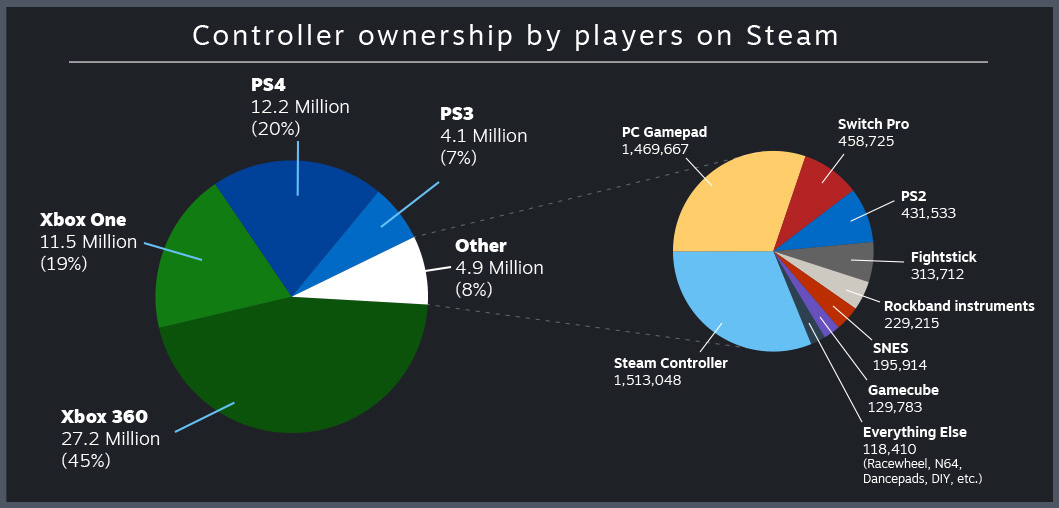
\includegraphics[width=\textwidth]{steamControllerStatistik.jpg}
    \caption{Verteilung von Besitz von verschiedenen Spielcontrollern auf der Plattform Steam\cite{SteamSteamNews2018}}
    \label{fig:controllerStats}
\end{figure}

\section{Algorithmen zur Abbildung der Rad-Daten in Controller-Eingaben}
Die Sensor-Daten der Gyroskope liefern die Winkelgeschwindigkeiten der Räder des Rollstuhls.
Diese sollen – wie bereits in Kapitel 5.3.1 beschrieben – auf die Eingabemöglichkeiten eines Spielcontrollers abgebildet werden, um sich im virtuellen Raum bewegen oder andere Eingaben tätigen zu können.
Die Abbildung erfolgt dabei auf einen Xbox360 Controller. Somit sind die abgebildeten Eingaben von jeder Software lesbar, die eine Xbox360 Controllerunterstützung implementiert haben.
Die in diesem Kapitel werden gelgentlich Aussagen getroffen die mit dem Emfinden des Nutzers zu tun haben oder von ihm abhängig sind.
Da subjektive Eindrücke nur schwer und unpräzise gemessen werden können, leidet dadurch an manchen Stellen die Aussagekraft.
Darüber hinaus konnten nur wenige Personen im Umkreis des Erstellers dieser Arbeit als Testperson verwendet werden, was zusätzlich einzelne Aussagen abschwächt.
Eine zukünftige Arbeit muss sich ausführlicher an diesen Stellen mit den Betreffenden Fragen befassen, und einen größeren diverseren Pool aus Testpersonen verwenden, um die Aussagekraft zu erhöhen.

\subsection{Abbildung auf einen Thumbstick}
Der direkte Weg die Raddaten in eine Eingabe umzuwandeln ist, diese auf jeweils eine Achse eines Thumbsticks abzubilden.
Dabei wird die x-Achse mit dem einen, die y-Achse mit dem anderen Rad dargestellt.
Vorteilig ist dabei, dass beide Achsen gleichzeitig angesprochen werden können.
Jedoch ist es schwieriger, die x-Achse zu bewegen, da sie anders ausgerichtet ist als das Rad, das gedreht wird.
Alternativ kann das Ansprechen einer Achse auch durch beide Räder passieren.
Dabei wird die x-Achse dann angesprochen, wenn sich die Räder gegeneinander drehen und die y-Achse, wenn sich die Räder miteinander drehen.
Damit wird eine intuitive Nutzung angestrebt.
Jedoch ist es dabei nicht mehr möglich, gleichzeitig den Cursor entlang beider Achsen zu bewegen, da sich die Räder nicht gleichzeitig mit- und gegeneinander drehen können.

\subsection{Abbildung auf einen simulierten Rollstuhl}
Da das im Rahmen dieser Arbeit entwickelte System darauf abzielt, in einem dreidimensionalen virtuellen Raum, auf einer Ebene zu navigieren, wird eine Abbildung benötigt, die die Position des Nutzers im virtuellen Raum verändert.
Da die Daten ohnehin von einem Rollstuhl kommen, liegt die Abbildung auf einen simulierten Rollstuhl nahe.
Um die Raddaten der zwei Räder auf eine Bewegung und Rotation eines Rollstuhls umzurechnen, muss erst festgestellt werden, welche Drehbewegungen zu welchen Rollstuhlbewegungen führt.
Dabei können vier vereinfachte Fälle unterschieden werden:

\begin{figure}[h]
    \centering
    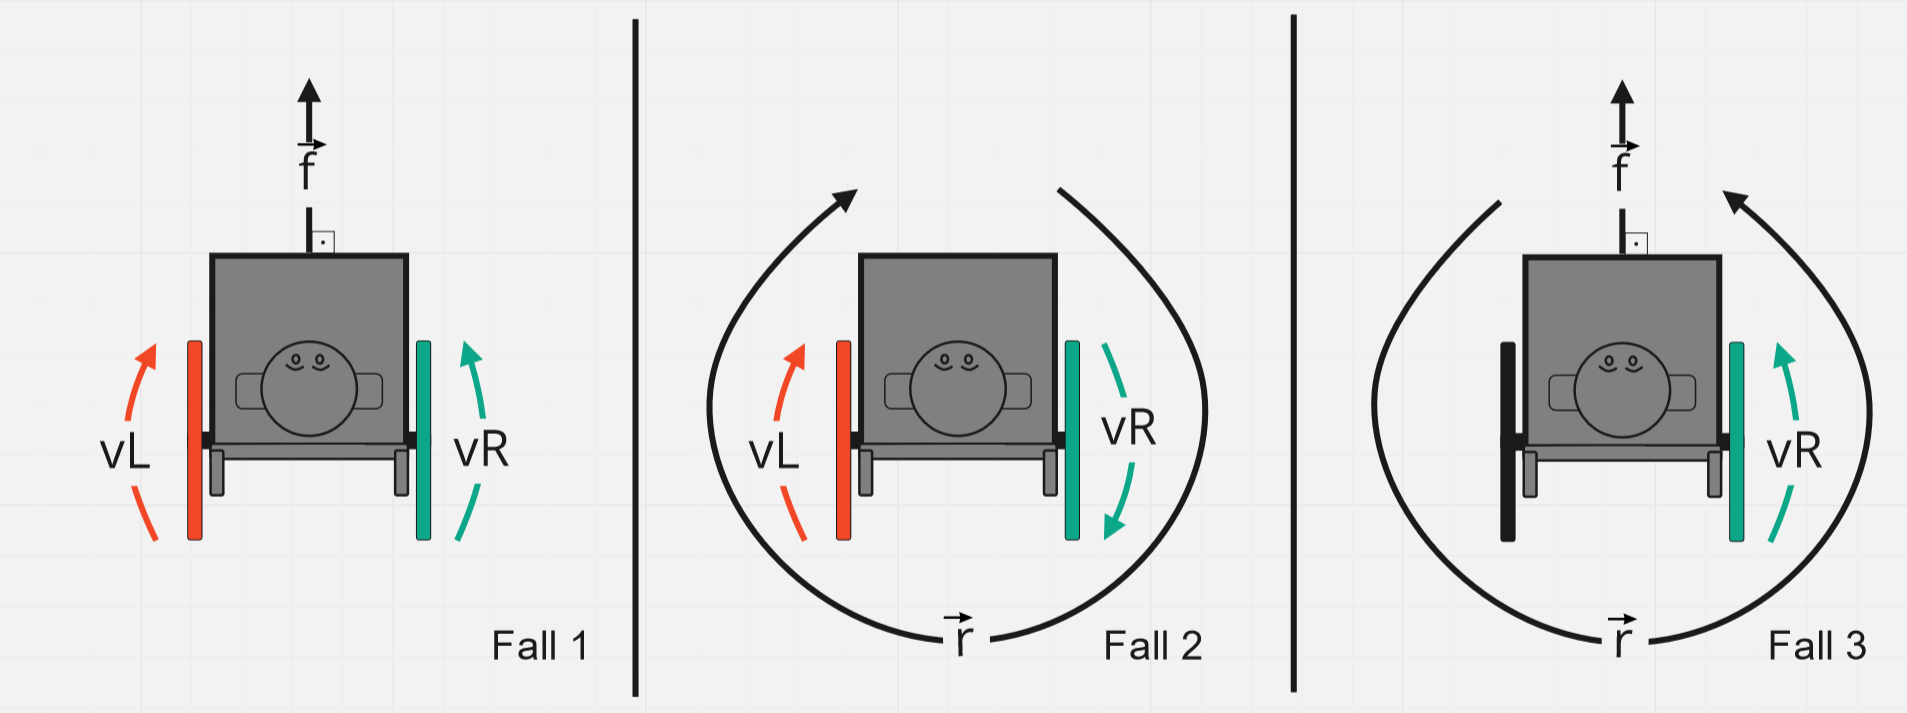
\includegraphics[width=\textwidth]{wheelchairCases.PNG}
    \caption{Die Bewegungs-Fälle des Rollstuhl aus der Vogelperspektive}
    \label{fig:wheelchairCases}
\end{figure}

\textbf{Fall 1:} Drehen sich die Räder mit gleicher Geschwindigkeit in dieselbe Richtung, so ruft dies eine Bewegung nach vorne oder hinten aus (Abbildung \ref{fig:wheelchairCases}, Fall 1).

\textbf{Fall 2:} Drehen sich die Räder mit gleicher Geschwindigkeit gegeneinander, so ruft dies eine Rotation um die eigene Achse hervor (Abbildung \ref{fig:wheelchairCases}, Fall 2).

\textbf{Fall 3:} Dreht sich nur ein Rad, so dreht sich dieses um das Stehende (Abbildung \ref{fig:wheelchairCases}, Fall 3).

\textbf{Fall 4:} Drehen sich die Räder unterschiedlich schnell, so muss die Bewegung zusammengesetzt werden aus den Bewegungskomponenten einer der ersten beiden Fälle und dem dritten Fall.

Im Folgenden wird die Berechnung der Bewegungsanteile aufgezeigt, bestehend aus Bewegung nach vorne/hinten und der Rotation um die eigene Achse:

\begin{align}
    \omega_L      & : \ \mathrm{Winkelgeschwindigkeit\ des\ linken\ Rades}\ [\si{\degree/\second}]  \\
    \omega_R      & : \ \mathrm{Winkelgeschwindigkeit\ des\ rechten\ Rades}\ [\si{\degree/\second}] \\
    m             & : \ \mathrm{Winkelgeschwindigkeit\ Minimum}\ [\si{\degree/\second}]             \\
    o             & : \ \mathrm{Overshoot}\ [\si{\degree/\second}]                                  \\
    d             & : \ \mathrm{Abstand\ Der\ R\ddot{a}der}\ [\si{\metre}]                          \\
    \vec{f}       & : \ \mathrm{Fortbewegungsvektor}\ [\si{\metre/\second}]                         \\
    \vec{r}       & : \ \mathrm{Rotationsvektor}\ [\si{\metre/\second}]                             \\
    \vec{f_{1,2}} & : \ \mathrm{Fortbewegungsvektor\ Fall1\ oder\ Fall2}\ [\si{\metre/\second}]     \\
    \vec{r_{1,2}} & : \ \mathrm{Rotationsvektor\ Fall1\ oder\ Fall2}\ [\si{\metre/\second}]         \\
    \vec{f_{3}}   & : \ \mathrm{Fortbewegungsvektor\ Fall3}\ [\si{\metre/\second}]                  \\
    \vec{r_{3}}   & : \ \mathrm{Rotationsvektor\ Fall3}\ [\si{\metre/\second}]
\end{align}

\begin{figure}[h]
    \centering
    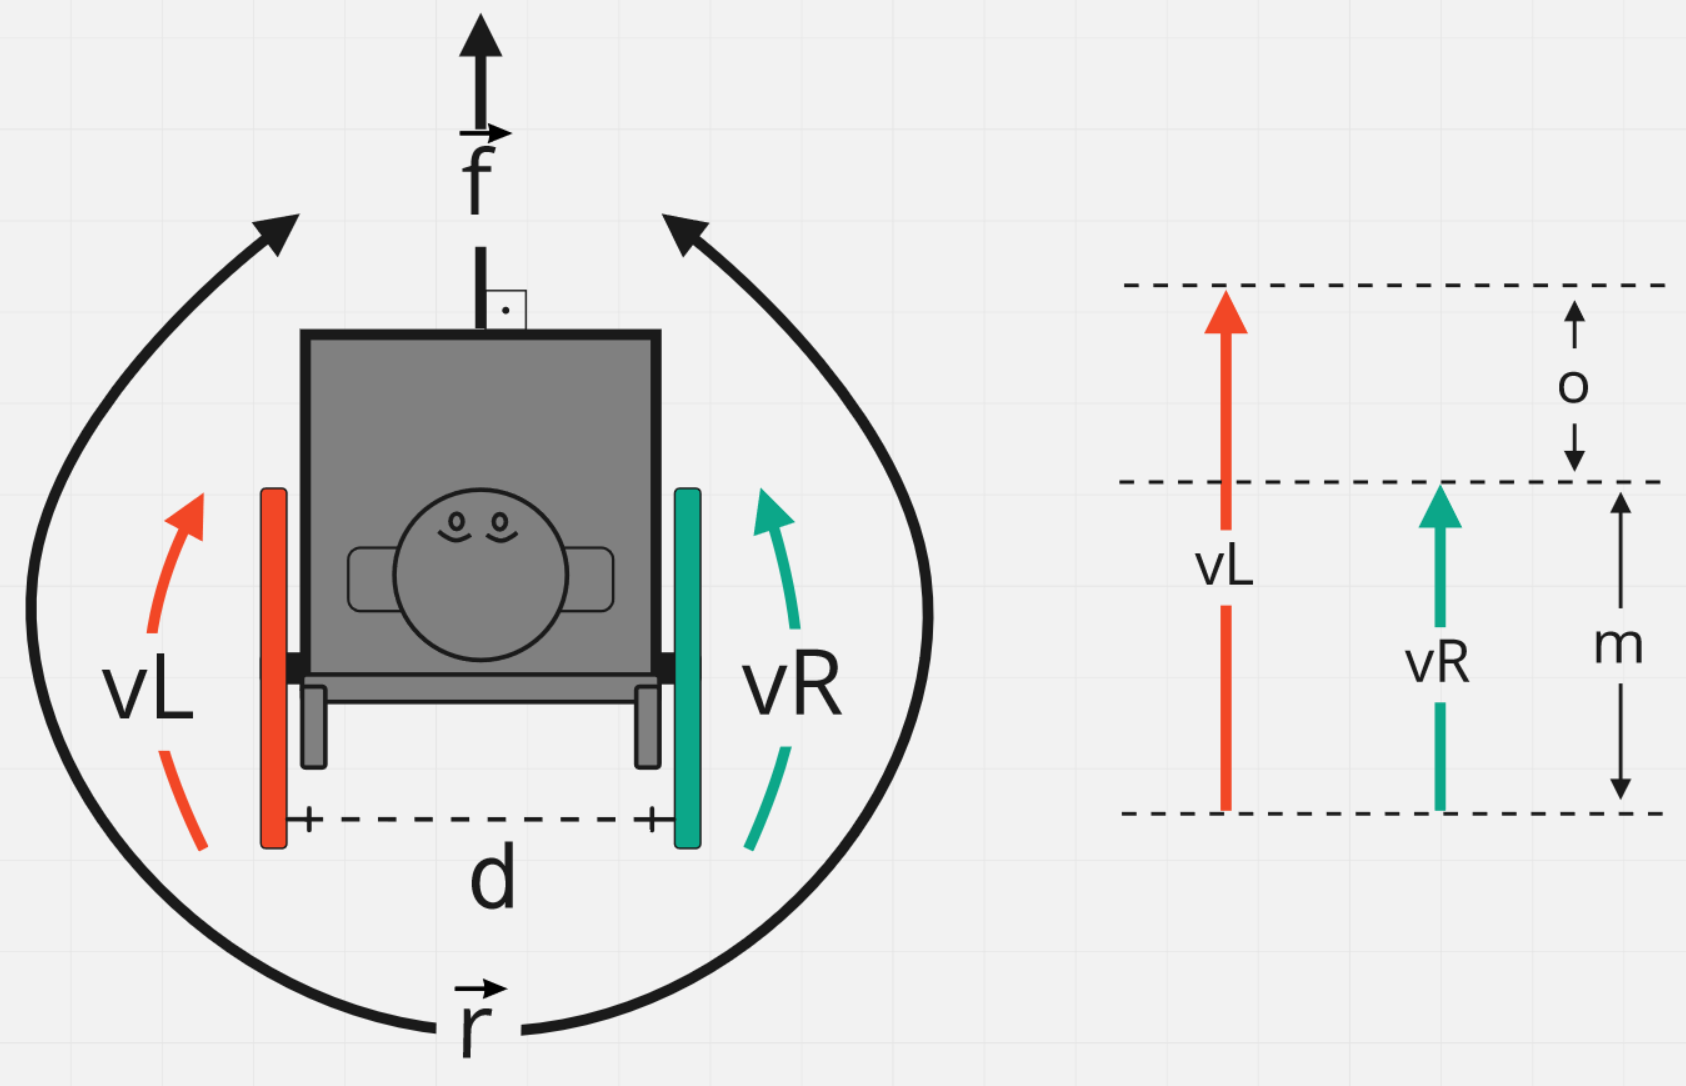
\includegraphics[width=0.75\textwidth]{WheelchairMath.PNG}
    \caption{Skizze des Rollstuhls aus der Vogelperspektive mit Bewegungsvektoren}
    \label{fig:wheelchairMath}
\end{figure}

Zunächst müssen die Rotationen der Räder dekonstruiert werden.
Dabei lässt sich die Rotation eines Rades in zwei Komponenten aufspalten (siehe Abbildung \ref{fig:wheelchairMath}).
Zum einen in den Minimum-Anteil $m$, den sich beide Räder drehen,
\begin{align}
    m = \min{(\left| \omega_L \right|,\left| \omega_R\right|)}
\end{align}

zum anderen in den Overshoot-Anteil $o$, den sich ein Rad schneller dreht als das andere.
\begin{align}
    o = \left|\left| \omega_L \right|-\left| \omega_R\right| \right|
\end{align}

\textbf{Fall 1:}
Die Bewegung nach vorne oder hinten (Fortbewegungsvektor Fall1 oder Fall2 $f_{1,2}$) ergibt sich in diesem Fall aus dem Anteil der Geschwindigkeit, mit denen sich beide Räder drehen.
Dabei dreht sich jedoch der Rollstuhl nicht.
\begin{align}
    \vec{f_{1,2}} = & \ m \\
    \vec{r_{1,2}} = & \ 0
\end{align}

\begin{figure}[h]
    \centering
    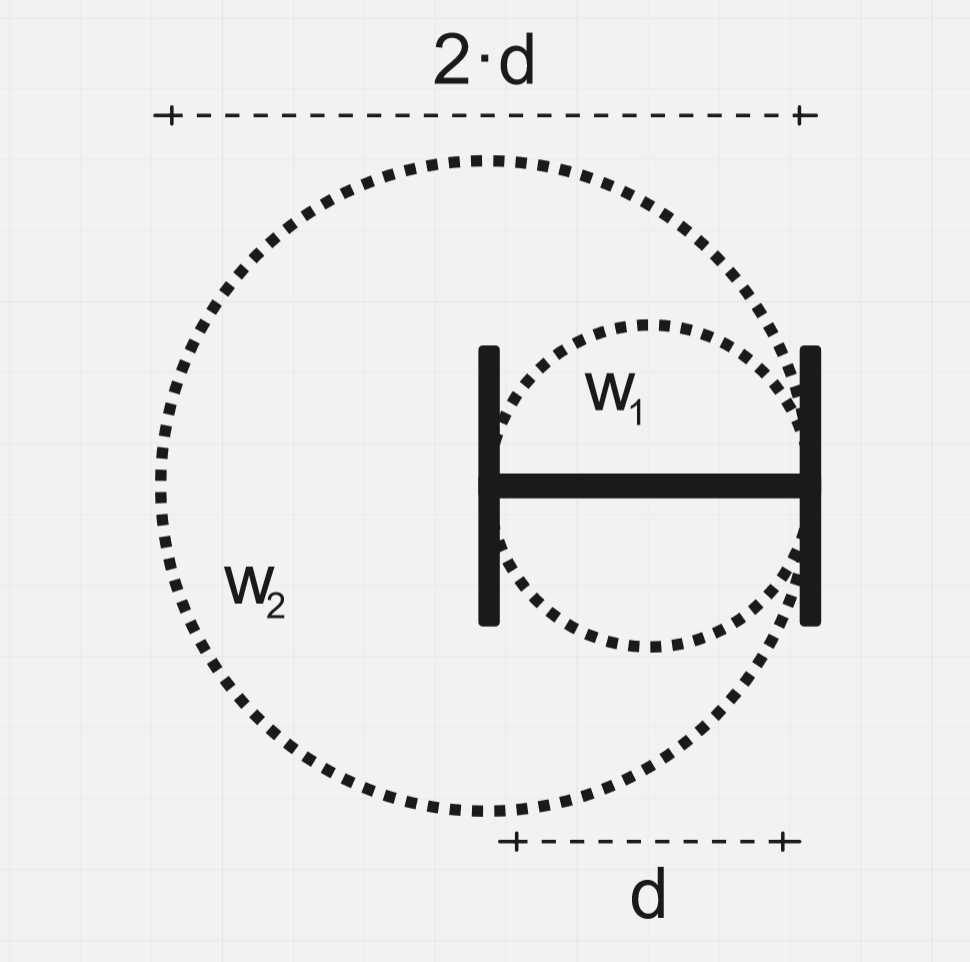
\includegraphics[width=0.5\textwidth]{wendekreis.PNG}
    \caption{Skizze des Rollstuhls aus der Vogelperspektive mit Wendekreisen}
    \label{fig:wendekreis}
\end{figure}

\textbf{Fall 2:}
Zur Berechnung der Rotation um die eigene Achse wird zunächst der Wendekreis $w_1$ benötigt.
Dieser Wendekreis ist abhängig vom Abstand der Räder $d$ und dessen Mittelpunkt liegt im Mittelpunkt zwischen den Rädern (siehe Abbildung \ref{fig:wendekreis}).
Anschließend wird mithilfe des Minimums $m$, das Verhältnis von $m$ zu $w_1$ errechnet, also wie viel vom Wendekreis gedreht wird.
Dieses Verhältnis muss zum Schluss mit $360$ multipliziert werden, um den resultierenden Winkel, beziehungsweise Rotationsvektor Fall1 oder Fall2 $r_{1,2}$, zu berechnen.
Bei dieser Bewegung verändert der Rollstuhl jedoch nicht seine Position.
\begin{align}
    w_1           & =            \ d \cdot \pi                  \\
    \vec{r_{1,2}} & =  \ \left(\frac {m} {w_1}\right) \cdot 360 \\
    \vec{f_{1,2}} & =  \ 0
\end{align}

\textbf{Fall 3:}
Bei diesem Fall gibt es einen Fortbewegungs- und einen Rotationsvektor ungleich null.
Da sich nur ein Rad bewegt, hat sich der Wendekreis vergrößert zu $w_2$.
Der Durchmesser von $w_2$ ist nun doppelt so groß wie von $w_1$, da das stehende Rad nun der Mittelpunkt des Wendekreises ist.
Jetzt wird der Overshoot $o$ (also der Anteil der Bewegung des Rades, das sich mehr als das andere dreht) ins Verhältnis gesetzt mit $w_2$ und erhält dadurch $\Theta$.
Verrechnet man $\Theta$ mit dem inneren Wendekreis $w_1$, so erhält man den Fortbewegungsvektor Fall3 $f_3$.
\begin{align}
    w_2 =       & \ 2 \cdot d \cdot \pi \\
    \Theta =    & \ \frac {o} {w_2}     \\
    \vec{f_3} = & \ \Theta \cdot w_1
\end{align}

Um den Rotationsvektor Fall3 $r_3$ berechnen zu können, muss $\Theta$ mit $360$ multipliziert werden.
\begin{align}
    \vec{r_3} = \Theta \cdot 360
\end{align}

Da die Berechnungen mit den absoluten Rotationswerten errechnet wurden, ist es notwendig anhand der Drehrichtungen beider Räder zu bestimmen, ob sich der Rollstuhl vor- oder zurückbewegt und ob er sich dabei nach links oder rechts dreht.
Die Drehrichtung ist immer dann links, wenn:
\begin{align}
    \omega_L < \omega_R
\end{align}

sonst ist sie rechts.
Es handelt sich um eine Vorwärtsbewegung, wenn:
\begin{align}
    \omega_L + \omega_R > 0
\end{align}

sonst ist es eine Rückwärtsbewegung.
Folgende Bedingungen können vernachlässigt werden, da sie in der Realität nur Auftreten wenn der Overshoot $o = 0$ ist und damit $\vec{f_3} = 0$ und $\vec{r_3} = 0$:
\begin{align}
    \omega_L =            & \ \omega_R \\
    \omega_L + \omega_R = & \ 0
\end{align}

\textbf{Fall 4:}
Bevor die zusammengehörenden Vektoren zusammengerechnet werden können, muss überprüft werden, ob $s_{1,2}$ und $r_{1,2}$ mithilfe des ersten oder zweiten Falls berechnet werden müssen.
Gilt folgende Bedingung, drehen sich die Räder gegeneinander und es wird Fall 2 benötigt.
Andernfalls gilt Fall 1.
\begin{align}
    (\omega_L > 0) \oplus (\omega_R > 0)
\end{align}

Anschließend können die Bewegungskomponenten addiert werden:
\begin{align}
    \vec{s} = & \ \vec{f_{1,2}} + \vec{f_3} \\
    \vec{r} = & \ \vec{r_{1,2}} + \vec{r_3}
\end{align}

Sind die Bewegungskomponenten berechnet muss final eine Abbildung dieser auf den Spielcontroller erfolgen.
Dabei bietet sich die y-Achse des linken-Thumbsticks an für den Fortbewegungsvektor $\vec{s}$ und die s-Achse des rechten Thumbsticks für den Rotationsvektor $\vec{r}$.
In vielen Anwendungen, im besonderen 3D-Videospielen, ist der linke Thumbstick für das Bewegen im Raum zuständig und der rechte für das Umschauen.

Berechnet man auf Grundlage der oben genannten Formeln die Bewegung des Rollstuhls, so stößt man auf folgendes Problem:
Da die Räder bei einer beabsichtigten Bewegung nach vorne meist mit leicht unterschiedlicher Geschwindkeit drehen, erfährt der simulierte Rollstuhl eine Ablenkung nach rechts oder links.
Eine Ausrichtung des Rollstuhls, die der Nutzer gezielt vorgenommen hat, um ein bestimmtes Ziel im virtuellen Raum zu erreichen, ist damit nichtig, da der Rollstuhl sein Ziel verfehlt.
Bildet man den Durchschnitt $v$ der Rotationen beider Räder und nutzt ihn anstelle vom $Minimum\ m$, so verhindert man die unbeabsichtigte Ablenkung.
\begin{align}
    \vec{v} = \frac {(\omega_L + \omega_R)} {2}
\end{align}

Verwendet man den Durchschnitt $v$ müssen die verschiedenen Fälle distinkt sein, da sonst das Wenden mit einem Rad nicht mehr möglich wäre.
Grund dafür ist der zusammenaddierter Mittelwert der Geschwindigkeiten des stillstehenden und des sich drehenden Rades.
Dieser würde anstelle einer Drehung zu einer Vorwärtsbegung führen.
Das Zusammenrechnen von Fall 1 oder Fall 2, mit Fall 3 darf also nicht geschehen.
Um dies zu realisieren, sind Bewegungszustände notwendig.
Auf Basis dieser kann entschieden werden, welcher Fall genutzt werden muss, um die resultierende Bewegung zu errechnen.
Im nächsten Kapitel wird darauf eingegangen, welche Bewegungszustände existieren und wie diese erkannt werden können.

\subsection{Bewegungszustände}
Um alle Bewegungszustand-Permutationen ermitteln zu können, muss festegestellt werden, dass sich ein Rad in drei Zuständen befinden kann: Still stehend, nach vorne drehend und nach hinten drehend.
Zwei Räder mit jeweils drei Zuständen ergeben dabei neun Bewegungszustände ($3^2 = 9$), welche in Abbildung \ref{fig:wheelstates} skizziert sind.

\begin{figure}[h]
    \centering
    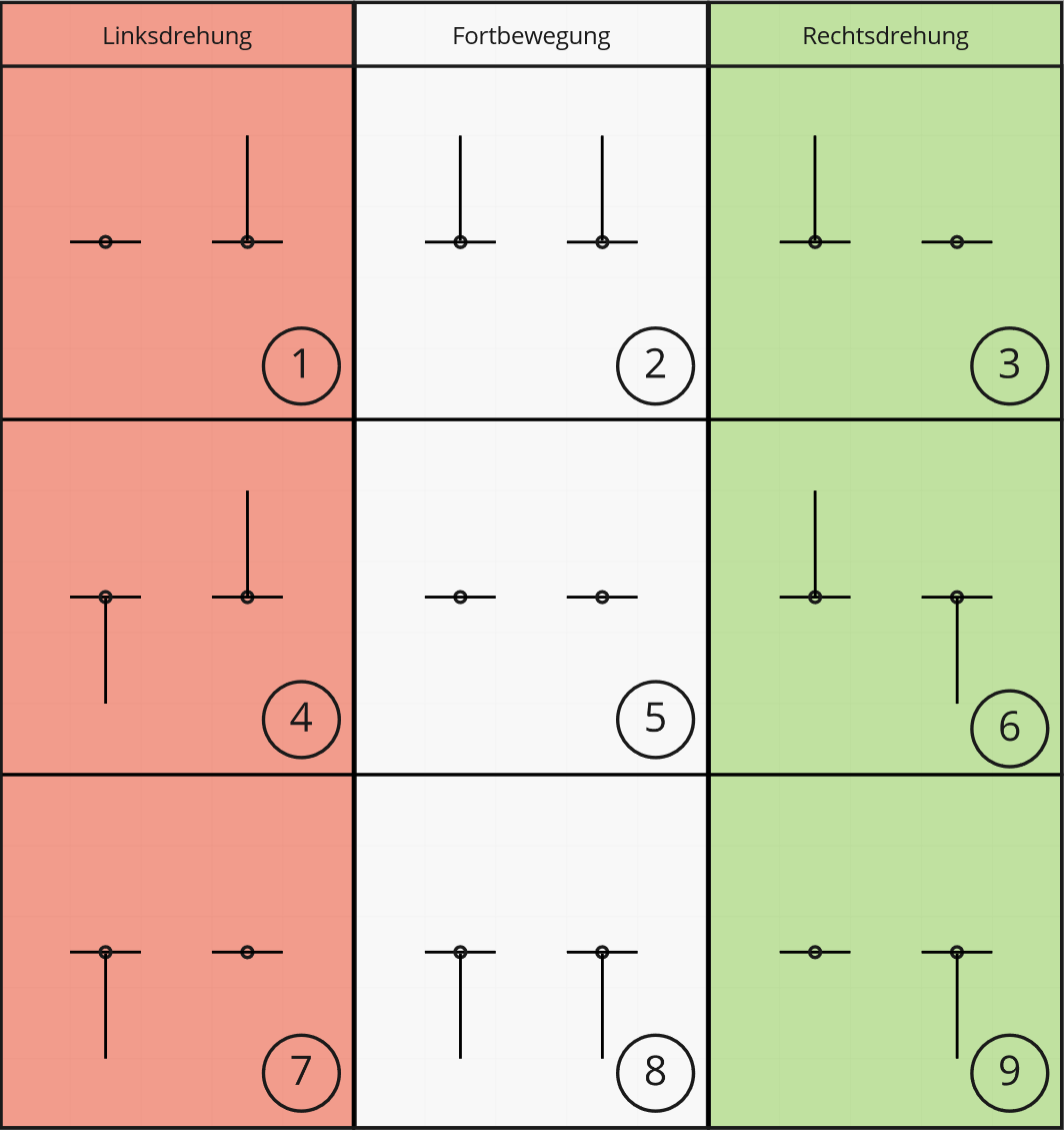
\includegraphics[width=0.75\textwidth]{WheelchairStates.PNG}
    \caption{Die neun Bewegungszustände eines Rollstuhls}
    \label{fig:wheelstates}
\end{figure}

Jedoch lässt sich die Menge von Bewegungszuständen in folgende disjunkte Teilmengen unterteilen:
\begin{itemize}
    \item \textit{Ruhezustand}: kein Rad dreht sich (5)
    \item \textit{Rotation um die eigene Achse}: Räder drehen sich gegeneinander (4, 6)
    \item \textit{Einzelradbewegung}: ein Rad steht still und ein Rad dreht sich (1, 3, 7, 9)
    \item \textit{Sichtachsenbewegung}: Räder drehen sich in dieselbe Richtung (2, 8)
\end{itemize}

Im Folgenden wird darauf eingegangen, wie diese Teilmengen-Zustände erkannt werden:
\begin{align}
    \omega_L & :\ \mathrm{Winkelgeschwindigkeit\ des\ linken\ Rades}  \\
    \omega_R & :\ \mathrm{Winkelgeschwindigkeit\ des\ rechten\ Rades} \\
    s        & :\ \mathrm{Schwellenwert}
\end{align}

\textbf{\textit{Ruhezustand}}\\
Der \textit{Ruhezustand} wird erreicht, wenn kein anderer Zustand zutrifft oder sich kein Rad dreht.
Da das oben beschriebene Rauschen abgeschnitten wurde, gilt der Ruhezustand wenn:
\begin{align}
    (\omega_L = 0) \land (\omega_R = 0)
\end{align}

\textbf{\textit{Einzelradbewegung}}\\
Wie beim Ruhezustand ist es auch hier möglich, darauf zu prüfen, ob ein Wert 0 ist.
Die einfachste Art und Weise dies zu prüfen, ist folgende Bedingung:
\begin{align}
    (\omega_L = 0) \oplus (\omega_R = 0)
\end{align}
Der Nutzer hat jedoch Schwierigkeiten, ein Rad vollständig ruhig zu halten.
Die Gyroskop-Werte überschreiten selbst bei kleinen Handbewegungen den Schwellenwert für die Rauschunterdrückung.
Dies führt zu unbeabsichtigten Eingaben.
Deshalb ist diese Methode unzureichend.
Führt man einen Schwellenwert $t$ ein, wird eine vom Nutzer unbeabsichtigte \textit{Einzelradbewegung} zuverlässiger unterdrückt:
\begin{align}
    (|\omega_L| < s) \oplus (|\omega_R| < s)
\end{align}

\textbf{\textit{Rotation um die eigene Achse}}\\
Die Bedingung, die gelten muss, wenn sich beide Räder gegeneinander drehen, ist identisch mit der Bedingung, welche schon im Kapitel \textit{Abbildung auf einen realistisch simulierten Rollstuhl} aufgestellt wurde.
Diese gilt nur, wenn \textit{Ruhezustand} und \textit{Einzelradbewegung} ausgeschlossen werden konnten, da nicht die Fälle abgedeckt werden, wenn $\omega_L$ oder $\omega_R$ 0 sind:
\begin{align}
    (\omega_L > 0) \oplus (\omega_R > 0)
\end{align}

\textbf{\textit{Sichtachsenbewegung}}\\
Der Zustand der Sichtachsenbewegung gilt dann, wenn sich die Räder in dieselbe Richtung drehen.
Damit ist dieser Zustand das logische Gegenteil der Bedingung \textit{Rotation um die eigene Achse}, vorausgesetzt es wurden \textit{Ruhezustand} und \textit{Einzelradbewegung} ausgeschlossen:
\begin{align}
    (\omega_L > 0) \Leftrightarrow (\omega_R > 0)
\end{align}

\subsection{Abbildung auf einen simulierten Rollstuhl mit zusätzlichen Interaktionen}
Werden, wie in Kapitel \textit{Abbildung auf einen simulierten Rollstuhl} erläutert, die Eingaben ausschließlich auf eine Rollstuhlbewegung abgebildet, so ist der Nutzer eingeschränkt in seinen Interaktionsmöglichkeiten.
Aktionen, wie ein Tastendruck auf dem emulierten Spielcontroller sind in diesen Fällen nicht möglich.
Jedoch können bestimmte Bewegungsmuster, die nicht zwangsläufig notwendig sind, genutzt werden, um weitere Interaktionen abzubilden.
Werden für das Drehen des Rollstuhls nur die Zustände genutzt, bei denen sich die Räder gegeneinander drehen (Abb. \ref{fig:wheelstates} Zustand 4 und 6), so bleiben vier Zustände übrig, die mit anderen Interaktionen belegt werden können (Abb. \ref{fig:wheelstates} Zustand 1, 3, 7, 9).
Bei diesen vier Mustern handelt es sich, um die Einzelradbewegungs-Zustände.
Diese können dann beispielsweise für das Drücken der Interaktionstasten des Spielcontrollers (\textit{A}, \textit{B}, \textit{X}, \textit{Y}) genutzt werden.

Bislang wurde die Anzahl der möglichen Interaktionen, durch die Anzahl der Bewegungszustände begrenzt.
Will man weitere Interaktionen abbilden, so bleibt nur die Geschwindigkeit mit der sich die Räder drehen oder die Zeit, um Anweisungen zu kodieren.
Bezieht man die Zeit in der sich Räder drehen mit ein, so könnte man das Morse-Alphabet abbilden. Dazu wäre nötig zwei Zustände zu definieren, wie zum Beispiel ein Rad kurz oder lange drehen.
Jedoch verkompliziert dies die Eingabe erheblich für den Nutzer, sodass diese Methode nicht weiter verfolgt wird.
Eine Alternative dazu ist die Geschwindigkeit mit einzubeziehen.
Teilt man den Wertebereich der Geschwindigkeiten eines Rades, so lässt sich in der Theorie die Anzahl der Bewegungszustände verdoppeln.
Dazu wird der Wertebereich zunächst mithilfe des Schwellenwertes $s = 100$ geteilt.
\footnotetext{Von einer weiteren Teilung ist abzuraten, da es sonst für den Nutzer schwierig wird, die Räder mit den gewünschten beziehungsweise notwendigen Geschwindigkeiten zu drehen.}
Die Unterscheidung zwischen langsamer und schneller Rotation ist jedoch intuitiv von jedem Nutzer begreifbar und umsetzbar.
Im Wertebereich der langsamen Bewegungen können nun Bewegungen, wie das Neigen des Kamerawinkels, abgebildet werden.
Dabei wurde sich für die Bewegungszustände 2 (Neigung nach oben) und 8 (Neigung nach unten) entschieden.
Für das Detektieren dieses neuen Teilmengen-Bewegungszustandes wird folgende Bedingung benötigt:

\textbf{\textit{Neigen}}
\begin{align}
    ((\omega_L > 0) \Leftrightarrow (\omega_R > 0))  \land (|\omega_L| < s) \land (|\omega_R| < s)
\end{align}

Unweigerlich geht dabei die Möglichkeit verloren, seinen Fortbewegungsvektor $s$ feiner einzustellen.
Es sind also keine langsamen Bewegungen nach vorne und hinten möglich.
Dafür hat der Nutzer die Möglichkeit, sich frei im Raum umschauen zu können.

\section{Optimierung der Detektion von Bewegungszuständen}
Für den Nutzer ist die korrekte Detektion von Bewegungszuständen entscheidend.
Werden unerwünschte Zustände ermittelt, führt dies zu fehlerhaften Eingaben, welche der Nutzer als störend empfindet.
Je mehr verschiedene Bewegungszustände voneinander unterschieden werden müssen, desto höher ist die Gefahr der Missinterpretation.
Abgesehen davon ist es nicht immer sinnvoll für alle Bewegungsmuster den Wertebereich zu teilen (wie in Kapitel \textit{Abbildung auf einen simulierten Rollstuhl mit zusätzlichen Interaktionen}).
Bewegungen, wie die \textit{Rotation um die eigene Achse}, wollen vom Nutzer entweder langsam und präzise oder schnell durchgeführt werden.
Nur in bestimmten Fällen, wie bei der Fortbewegung, kann es sinnvoll sein, den Wertebereich zu teilen.
So ist die Anzahl der tatsächlich sinnvollen Bewegungsmuster kleiner als die theoretisch denkbaren.
Es muss bei jedem Zustand und jeder Interaktion abgewogen werden, ob eine Teilung des Wertebereichs sinnvoll erscheint, oder den Nutzer behindert.
Trotz der verringerten Anzahl an Bewegungsmustern, sind beim Testen der \textit{Abbildung auf einen simulierten Rollstuhl mit zusätzlichen Interaktionen} zwei primäre Probleme beobachtet worden, bei denen fehlerhafte Eingaben getätigt werden.
Zum Testen des Systems und Aufnehmen der Daten wurde \textit{Counter-Strike: Global Offensive} verwendet.

\subsection{Unbeabsichtigtes Betätigen von Interaktionstasten}
In den ersten Testreihen wurde für die Detektion von einer \textit{Einzelradbewegung} und dem Teilen des Wertebereichs in schnelle und langsame Bewegungen derselbe Schwellwert $s = 100$ verwendet.
Unter Verwendung dieser Methode kommt es beim Anfahren oder Bremsen (\textit{Sichtachsenbewegung}) zum unbeabsichtigten Betätigen von Interaktionstasten.
Da sich die Räder nicht mit derselben Geschwindigkeit drehen, gibt es ein kurzes Zeitintervall, in dem ein Rad unter dem Schwellwert und ein Rad über dem Schwellenwert liegt.
Aus der Abbildung \ref{fig:1_threshold} ist abzulesen, dass für dieses Zeitintervall die Bedingung der \textit{Einzelradbewegung} gilt, sodass eine Interaktionstaste betätigt wird.

\begin{figure}[h]
    \centering
    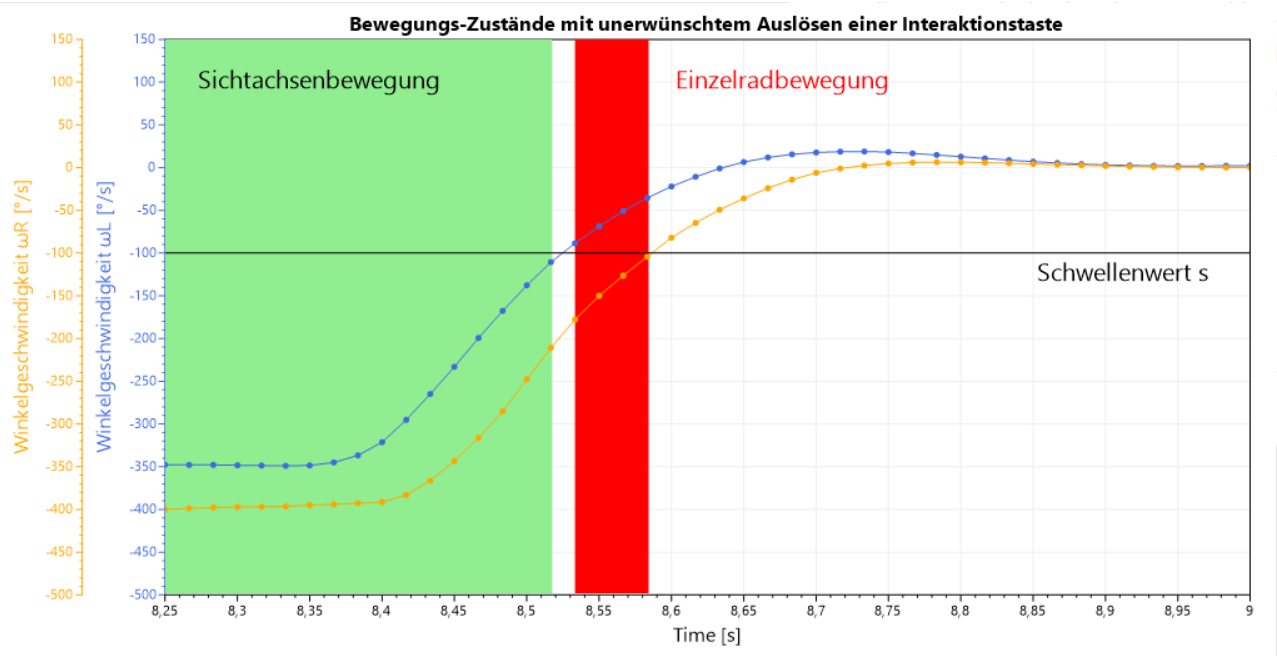
\includegraphics[width=0.75\textwidth]{1threshold.PNG}
    \caption{Bewegungs-Zustände mit unerwünschter \textit{Sichtachsenbewegung}}
    \label{fig:1_threshold}
\end{figure}

Dieses Problem lässt sich über das Einführen eines neuen \textit{Einzelradbewegung} Schwellenwertes beheben.
Wählt man für diesen einen geringeren Wert $s_1 = 25$ als für den Schwellwert für das Teilen des Wertebereichs $s_2$, entsteht eine Pufferzone.
Beim Beschleunigen überschreiten die Gyroskop-Werte zunächst nacheinander $s_1$. Anschließend überschreiten die Werte nacheinander $s_2$.
Solange beide Werte in der Pufferzone sind, kann weder eine \textit{Einzelradbewegung} noch eine \textit{Sichtachsenbewegung} detektiert werden (siehe Abbildung \ref{fig:2_threshold}).

\begin{figure}[h]
    \centering
    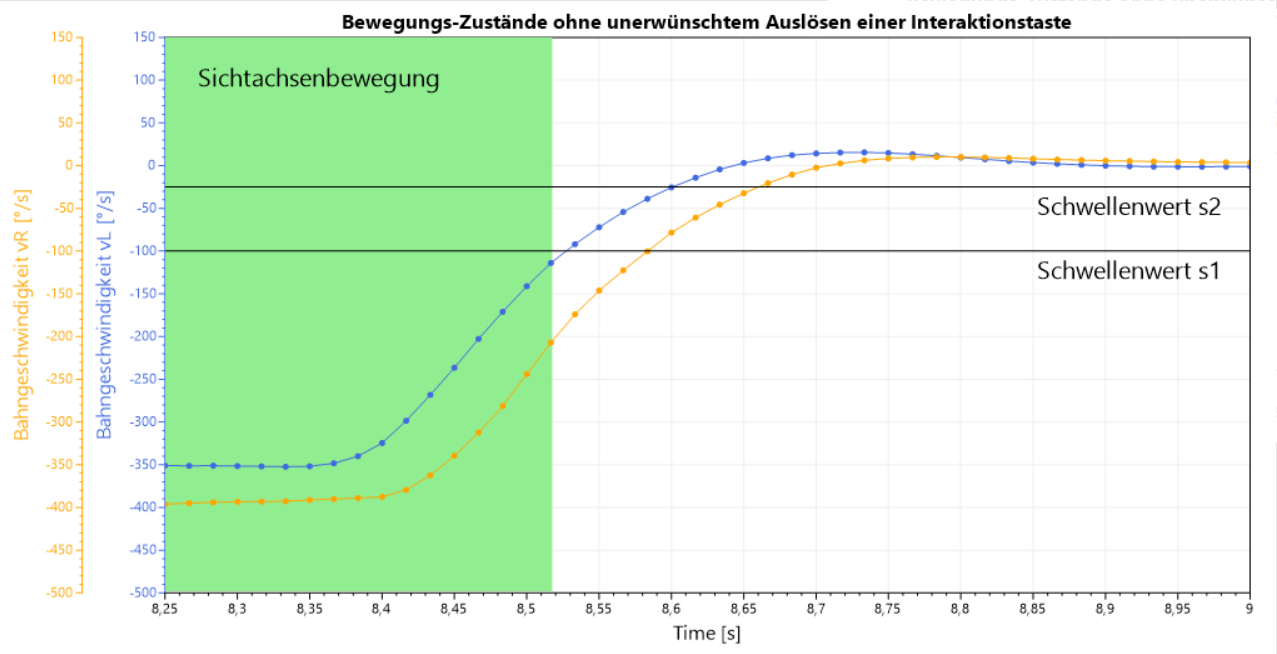
\includegraphics[width=0.75\textwidth]{2threshold.PNG}
    \caption{Bewegungs-Zustände ohne unerwünschter \textit{Sichtachsenbewegung}}
    \label{fig:2_threshold}
\end{figure}

Durch das Einführen der neuen Schwellenwerte müssen folgende Teilmengen-Bewegungszustände erweitert werden:

\textbf{\textit{Einzelradbewegung}}
\begin{align}
    ((|\omega_L| < s_1) \oplus (|\omega_R| < s_1)) \land ((|\omega_L| > s_2) \oplus (|\omega_R| > s_2))
\end{align}

\textbf{\textit{Sichtachsenbewegung}}
\begin{align}
    ((\omega_L > 0) \Leftrightarrow (\omega_R > 0)) \land ((|\omega_L| \geq s_2) \land (|\omega_R| \geq s_2))
\end{align}

\textbf{\textit{Neigen}}
\begin{align}
    ((\omega_L > 0) \Leftrightarrow (\omega_R > 0)) \land (|\omega_L| < s_2) \land (|\omega_R| < s_2)
\end{align}

\subsection{Unbeabsichtigtes Neigen beim Anfahren}
Beim Anfahren oder Bremsen (\textit{Sichtachsenbewegung}) wurde beobachtet, dass für ein kurzes Zeitintervall der Kamerawinkel unbeabsichtigt geneigt wird.
Ähnlich wie beim vorangegangenen Problem wird auch hier beim Übergang von einem Zustand zum Nächsten ein unerwünschter Zwischenzustand erreicht.
In diesem Fall gibt es beim Beschleunigen einen kurzes Zeitinterval in dem die Rollstuhl-Software im \textit{Neigen}-Zustand ist, da $|\omega_L|$ und $|\omega_R|$ beide unter dem Schwellenwert $s_2$ sind (siehe Abbildung \ref{fig:ohneAcc}).

\begin{figure}[h]
    \centering
    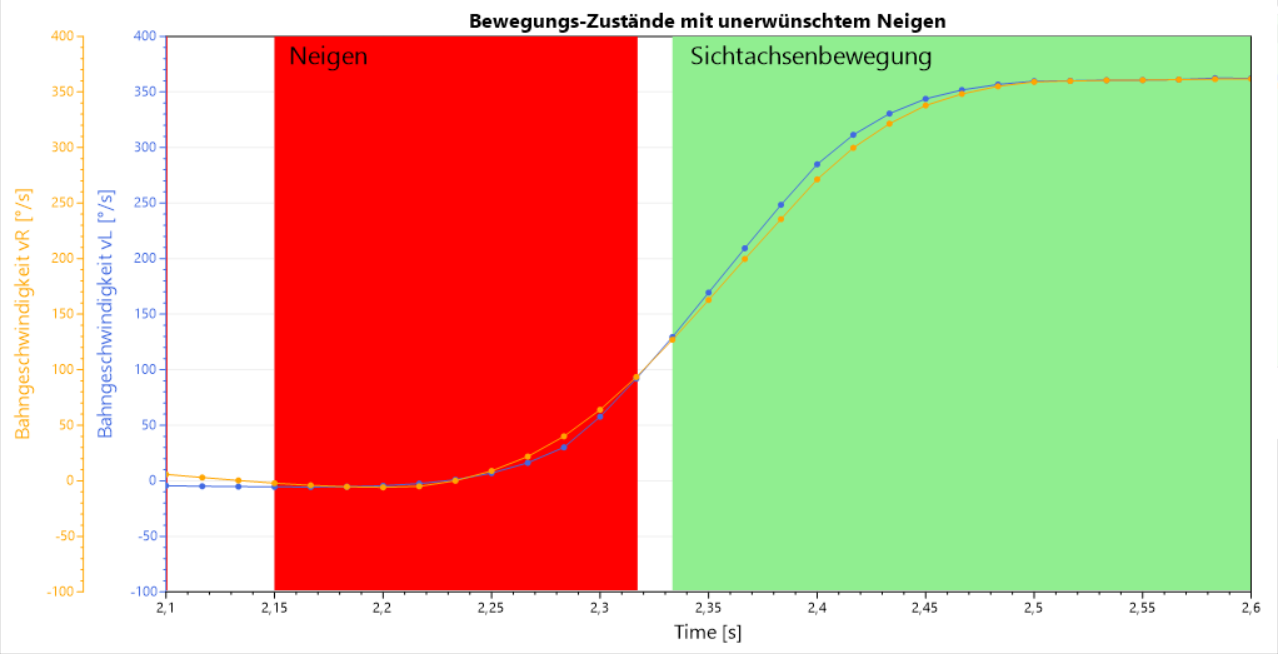
\includegraphics[width=0.75\textwidth]{ohneAcc.PNG}
    \caption{Bewegungs-Zustände mit unerwünschtem \textit{Neigen}}
    \label{fig:ohneAcc}
\end{figure}

Da die Fehldetektion immer dann auftritt, wenn sich die Geschwindigkeit der Räder ändert, ist der hier verwendete Lösungsansatz, die Bedingung des Neigungs-Zustandes zu erweitern.
In dieser wird nun auch abgefragt, ob die Summe der Änderungsraten $a$ der Gyroskope unter einem neuen Schwellenwert $s_3$ liegt.
Haben die Räder ihre Zielgeschwindigkeit erreicht, fällt die Änderungsrate unter $s_3$, sodass der nächste korrekte Zustand detektiert werden kann.
In den Tests hat sich $s_3 = 15$ als ein akzeptabler Wert herausgestellt, wie aus den Diagrammen abzulesen ist.
Für die Berechnung der Änderungsrate wird folgende Berechnung verwendet:
\begin{align}
    a = |(\omega_{L,[1]} - \omega_{L,[0]})| + |((\omega_{R,[1]} - \omega_{R,[0]})|
\end{align}

Die Bedingung des Teilmengen-Zustands \textit{Neigen} muss wie folgt ergänzt werden:

\textbf{\textit{Neigen}}
\begin{align}
    ((\omega_L > 0) \Leftrightarrow (\omega_R > 0)) \land (|\omega_L| < s_2) \land (|\omega_R| < s_2) \land (a < s_3)
\end{align}


\begin{figure}[h]
    \centering
    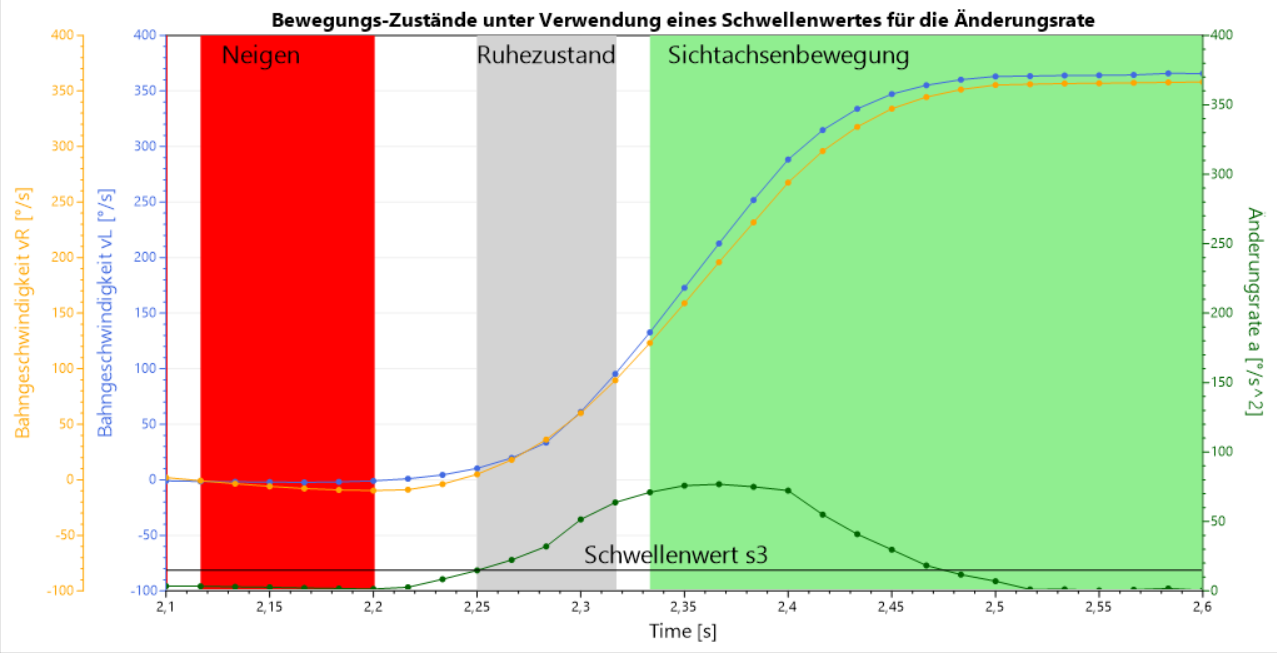
\includegraphics[width=0.75\textwidth]{mitAcc.PNG}
    \caption{Bewegungs-Zustände unter Verwendung eines Schwellenwertes für die Änderungsrate ohne unerwünschtem \textit{Neigen}}
    \label{fig:mitAcc}
\end{figure}

Aus der Abbildung \ref{fig:mitAcc} ist abzulesen, dass zwischen dem \textit{Sichtachsenbewegung}-Zustand und dem \textit{Neigen}-Zustand nun ein kurzer Ruhezustand existiert.
Diese Verzögerung bei der Fortbewegung ist vom Nutzer kaum bis gar nicht wahrnehmbar.
Im gezeigten Beispiel beträgt diese nur etwa 70ms.
Jedoch ist anzumerken, dass diese Methode vor allem bei ruckartigen Bewegungen funktioniert, da besonders dann die Änderungsrate schnell einen registrierbaren Ausschlag hat.
Verändert sich die Geschwindigkeit nicht schnell genug, kann es immer noch zu registrierbaren Neigungen kommen.

